%Tutkimusaineisto ja -menetelmät
\section{3D scanning rig implementation}

\subsection{Functional specification} % {{{

The implementation was specified to be easy to use, portable, flexible and available for both 3D and 4D cases, 4D being a nice-to-have feature.
Portability and open design was also considered to be important.
By documenting the selected hardware and its structure, and writing control code in a generic way, it is hoped that the design could be reimplemented and/or refined by others too.

There is a wide variety of different consumer grade digital cameras.
Some of the main differences are dicussed below.

% }}}

\subsubsection{Features} % {{{

Some of the above stuff goes here

% }}}

\subsubsection{Practicalities} % {{{

A general-purpose reconstruction rig has remarkably many practical matters to consider when comparing to the pure mathematical side.
A mobile rig should be light enough to carry and set up, but it should be rigid enough to give proper quality pictures and hold its calibrated configuration.
Distance to the photographed target should not be too short in order to not annoy human targets, but a too large setup is difficult to build and needs lots of space.
When capturing video, the frames should be synchronized among cameras as described in \ref{sec:somethingaboutvideosync}, which might not be possible with a reasonable budget.

% or \subsection{Data recording}

- lens distortion?
- rigid base, motion blur
- baseline width, focus, depth, fstop etc
- compression artifacts are nasty (edge detectors go wild etc.)

% }}}

\subsection{Camera comparison} % {{{

not considered: weatherproofing, lcd/viewfinder/user interface, mirror blackout, autofocus, etc

The section \ref{sec:cameratypes} presents in more detail the properties necessary for reconstruction.

Reliability on configurability and controllability was considered important.
Cheaper cameras fit more into a budget, but they might not be properly controllable.
External shutter release mechanisms have been researched more on DSLRs;
the manufacturers do not provide official specifications of the release connector pinouts, but they have been reverse-engineered for many models by individual tinkerers.
Zoom-only lenses and lack of raw processing, fast processors, manual modes etc.~leave cheaper compact cameras out of the comparison.
More expensive models do have comparable features, but their prices rise into the same range as with DSLRs that are more understood.

Canon DSLRs have been used previously on commercial setups [infiniterealities, ten24, capture lab likeness capture rig (ea sports/fifa example), remedy].
Commercial video capture setups use specialized machine vision devices and partly custom software to export data into suitable format.

Machine vision devices need several high performance computers for reliable multi-camera capture.
Where each camera outputs approximately 1 Gbit/s of data, approximately one hard disk per camera is needed if the capture is long enough and does not fit in a computer's RAM, increasing the system cost and complexity.
Best mechanical hard disks have sequential write speed that just exceeds 1 Gbit/s;
newer solid-state disks (SSD) generally are two to four times faster.

For covering all the bandwidth, an expansion card would be needed per camera, count depending on the camera protocol. According to specifications, USB 3.0 has a maximum transmission rate of 5 Gbit/s, Camera Link supports 5.44 Gbit/s in base and full configuration, FireWire up to 3,2 Gbit/s and GigE only 1 Gbit/s.
Additionally, actual data transfer speeds are less than the theoretical max rate advertised because of protocol and operating system overhead.
Most PC motherboards can accommodate only a few cards, requiring several PCs.

\begin{itemize}
\item CMOS/CCD sensor. CMOS suffers from rolling shutter in video mode, while CCD is more expensive and rare.
\item Resolution and sensor size. Higher resolution covers more detail, until airy disk size is reached. Larger sensor is more sensitive to light and therefore results in lower noise.
\item Lens quality. High resolution is only useful if the lens is sharp enough to fully use the pixel count.
\item Dynamic range, i.e. bit depth of the processing pipeline. JPEG pictures have only 8 bits per color channel, whereas DSLRs and industrial cameras use more, often 12 to 14 bits per pixel (in raw image, that contains the raw bayer pattern before interpolation)
\item Continuous speed. Controlled by many factors, the rate at which full-size pictures can be taken; image processing speed and memory card write speed have most effect.
\item Dust reduction. If enabled for some consumer cameras, it is implemented as high-frequency vibration of the sensor on camera bootup. Because it moves the sensor, it may affect calibration. (Not sure.)
\item Optical stabilization works by moving a glass element inside the lens or the sensor itself, effectively moving the image on the sensor, having a bad effect on calibration.
\item Video frame rate, resolution and compression. Cameras that support raw usually only use raw for still pictures and compress the video, as raw video is often unnecessary in the consumer market and uses lots of space. For image processing, each frame should be as little compressed as possible. Some DSLRs support ALL-I format, which contains only full keyframes (still compressed, but not predicted from other actual frames).
\item Usb speed. Retrieving saved image or video data takes less time for faster interfaces.
\item External flash. Practically all system cameras can be wired to an external flash lamp; only some compact cameras support this. Industrial cameras are externally triggered and require custom wiring.
\item Shutter lag. Lag measured between ordering the camera to take the picture to the actual moment where exposure starts should be consistent, and preferably small.
\item Weight and size. A smaller and lighter camera requires less bulky support structures.
\item Price. With a fixed budget, cheaper cameras can cover a larger area of the subject at a time because more cameras fit in the budget.
\item Availability. For an easily replicable system, it should be simple to purchase the hardware.
\item Configurability. Obviously, aperture, shutter speed and others should be manually controllable and repeatable without automatic features.
\item Low noise. Sensor noise shows immediately in the image quality, complicating correspondence and others.
\item Remote trigger. All DSLRs have usually wired and wireless remote shutter releases; some machine vision cameras have optionally an external logic-level trigger input in addition to one that is set by the protocol. Some protocols may have global commands to send throughout a group of cameras. (FireWire?) Otherwise, software trigger suffers from jitter from operating system and protocol randomness.
\end{itemize}

Prices for compact cameras that have the required features go up to the same price range as DSLRs or even higher, i.e. 500 EUR and up.

Having a much smaller production rate than larger manufacturers that target consumers (such as Canon or Nikon), industrial cameras have a broad price range from a few hundred euros to thousands, well correlated with pixel count and frame rate.
Lens prices for industrial C-mounts are moderate, at around 200-300 EUR.

% }}}

\subsection{Selected cameras} % {{{

Precise information on all hardware used can be found in appendix \ref{app:hardwareused}.

A DSLR is a good choice because of moderate price compared to image quality, and availability of usable software.
Canon was chosen because of previously acquired knowledge of the manufacturer, previously proven work using the same maker [infiniterealities, ten24, capture lab likeness capture rig (ea sports/fifa example), remedy] and firmware customizability \cite{magiclantern}. % this also above in practicalities

\subsubsection{Canon EOS 700D DSLR}

Canon EOS 700D body (or Rebel T5i in US), introduced in 2013, is among the newest of Canon's consumer range, with a price at about 600EUR.
Key features important for reconstruction are shown in table \ref{tab:eos700dfeatures}.

\begin{table}[h]
	\centering
	\begin{tabular}{l l}
		Sensor type & CMOS\\
		Sensor size & APS-C 22.3 x 14.9 mm\\
		Pixel size & 4,3 x 4,3 $\text{\si\micro m}$\\
		Image resolution & 5184 by 3456 pixels (17,9 million) \\
		Processor & Canon Digital Imaging Core (DIGIC) 5\\
		Bits per pixel & 14\\
		Shooting speed & five frames per second\\
		Video mode & 1080p in 30 FPS or 720p in 60 FPS
	\end{tabular}
	\caption{Canon EOS 700D key features}
	\label{tab:eos700dfeatures}
\end{table}

Large pixel count combined to a sharp lens is useful in bringing in a lot of detail.
The sensor's pixel size is not unnecessarily small but not as large as in full frame cameras.
Dynamic range with 14 bits per pixel is more than enough, as most reconstruction programs use 8-bit JPEG images.
The 5 FPS continuous speed for full-size images can be used for testing high resolution motion, but the video abilities should be reasonable for motion testing.
Raw video recording is also possible with modified camera firmware.

The sensor is labeled ``Hybrid CMOS'', a new Canon's technology that embeds phase-detection autofocus pixels in the sensor for fast continuous autofocusing in video mode.

The camera also features a tilting LCD screen that has provided to be useful when looking the camera from the front.

Older models of the same product line can still be found in the market, such as 650D or 600D. 700D has a newr processor and thus faster processing speed, faster memory card controller and others. Resolution of the sensor has stayed same since 550D, introduced in 2010.
At the same time also cheaper new models are available, such as 1200D. At a reduced price, less processing power is provided, resulting in slower operation but otherwise the cameras share mostly same features.

An important consideration was the ability to use the third-party Magic Lantern firmware add-on;
it was originally designed for improved user interfaces for video recording, but has been extended for other features too.
Firstly, it provides experimental support for raw video recording and other hacks; additionally, being open source, it can be modified for any custom purposes, such as multi-camera synchronization aids.

The camera uses SD cards for mass storage. A high-speed class 10 UHS-I card was selected; manufacturer claims 45 MB/s write speed.

Additionally, AC power adapters were chosen to operate the cameras without the need for charging batteries.
Canon sells adapters that plug in the camera's battery holder, providing continuous power at the expense of an additional cable per camera.

\subsubsection{Canon EF 50mm f/1.8 II}

Canon's EF-mounting 50mm f/1.8 II lens (priced at about 110 EUR), shown in figure \ref{fig:canonef50mmlens} is commonly known for its excellent, sharp image quality at a low price.
The lens was introduced in 1990.
Despite the poor plastic build quality, its glass is very good and it is well known as one of the best portrait lenses.
The lens changes between autofocus and manual focus modes with a mechanical switch, and the focus ring in manual focus mode is loose enough that it might need to be locked with tape if left on for a long time shooting to hold its position for a calibrated setup.

\simplefig{h}{%
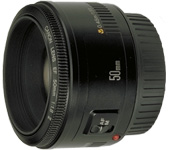
\includegraphics[width=0.4\textwidth]{gfx/canonef50mm-1}
%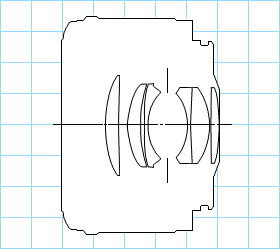
\includegraphics[width=0.4\textwidth]{gfx/canonef50mm-2}
}{fig:canonef50mmlens}
{Canon EF 50mm f/1.8 II, a fixed focus lens chosen for the rig}

% }}}

\subsection{Hardware construction} % {{{

\subsubsection{Mechanical choices}

With flexibility and mobility as requirements, the system should be built of removable parts that need no modifications to the environment, such as screwing bolts to nearby walls.
The separate parts should be small enough for transportation, but large enough for rigidity and build simplicity.

Two major designs were considered: a frame consisting of industrial aluminium profile system, or individual tripod stands available in most photography stores meant for supporting lights.
For connecting the cameras, a custom profile could make use of also custom built parts; also, photography stores sell screws and clamps meant for connecting cameras, lights and other hardware.

Extruded aluminium profiles such as those by MiniTec, Item or Bosch Rexroth consist of square tube with a T-shaped slot running along each side, sometimes called T-slot systems.
The profile systems are commonly used in assembly lines and other automation installations in factories, but also in smaller assemblies; mechanical details vary by manufacturer but most supply a large catalog of connection brackets, hinges, screws etc. that allow much flexibility in the frame design.
A hobbyist-targeted manufacturer is OpenBuilds that targets open source projects, such as 3D printers and CNC routers.
The cost of such profile is around 10-20 EUR/m, with varying prices for connecting pieces; availability varies by supplier.

Ready-made light or speaker stands come in a variety of sizes and share a common design with an extendable center rod and three legs.
Typical light stands have an universal mount in one end of the rod for fastening a lamp.
Speaker stands do not have a similar standard; in general, they are heavier and thicker to support a larger mass.
Most photography studio stores offer a variety of light stands; some have a similar range of speaker stands.

A custom aluminium profile system has its benefits in rigidity and positional flexibility, because it can be built in any shape.
On the other hand, one rigid shape is more difficult to modify when such a change is needed.
Standard light or speaker stands are good because of their availability in normal stores.
A stand consisting of mostly round rods lacks flat surfaces and slots that could be used for fastening parts together.
For that purpose, special clamps and ball heads are sold separately.

Machine vision cameras do not generally use same tripod screws aimed for consumer market, but are screwed on with custom bases.

\subsubsection{Selected design}

The selected method was to use ready-made, heavy duty lighting stands.
Millenium LST-310 (sold by Thomann) is a sturdy three-legged lighting stand with a pole that can be zoomed several meters high.
Additionally, it has a horizontal bar at the top that was removed as useless.
The same tripod is used in other projects in the same lab and was found useful.
The relatively heavy weight (10 kg) makes the support structures steady. % FIXME weight

Four of these stands were bought, and testing was done with three, with three cameras in each.

For flexibility, each camera should be able to rotate in at least to horizontal or vertical pose, with arbitrary aiming position.
For that, Manfrotto 494 ball heads were used, connected to the tripod rod with Manfrotto 035 Super Clamps. Figure \ref{fig:TODO}.

The total structure of all nine cameras divided in three supports (figure \ref{fig:TODO}) takes up relatively little space, and is flexible enough to move around for any office-size subject.

Wires and power adapters are fastened to the stand legs in long-term use to reduce wires running on the floor.

% }}}

\subsection{Remote shutter synchronization} % {{{

For a rig with dynamic subjects, the cameras have to be synchronized to record the same data, as described in \ref{sec:videosomething}.
Photo synchronization was done with a remote mechanism provided by the camera, by driving the remote control of all cameras simultaneously.
In video recording mode, the same remote wire can be used with 3rd-party firmware to start recording.

% }}}

\subsubsection{Canon remote trigger} % {{{

The selected Canon EOS 700D has an input port for focus and shutter release, in addition to the integrated shutter button.
The camera uses a standard 2,5 mm sized stero jack for connecting external remote controllers.
Wired and wireless electronic remotes are available in the market, but no standard devices for triggering several cameras are available. % seem to exist.
Fortunately, the triggering method is widely researched among hobbyists; it is well enough documented in the internet.

The remote release jack is a three-contact connector, where one pin serves as a common ground, and connecting another pin to the ground triggers the camera's focus button, and the third pin releases the shutter when connected to the ground.
Luk from doc-diy.net \cite{docdiy} describes the camera's trigger circuit internals; the wires supply some current that flows back to the camera via the ground pin, which is why the cameras should be separated from each other electrically insteaad of connecting the similar remote wires of all cameras together.
A commonly used method among the DIY community is to use opto-isolators to control each camera individually, isolated from the shared control circuit.

An opto-isolator provides a galvanically separated switch that can be used to electrically ``connect'' the release wire to the camera's ground such that no electrical signal path is shared between the cameras.
The switch is commonly a phototransistor that is triggered externally by the light transmitted from a LED.
Both the phototransistor and the LED are installed in a opaque plastic housing.
As an example, the opto-isolator device used in this work is shown in figure \ref{fig:opto-isolator}.
The particular device works in open collector setting, exposing an open collector pin and an emitter of the transistor.
Another popular setting is powered device that outputs a voltage signal from a power supply.

% TODO: fig:opto-isolator in physical form and in a schematic diagram next to each other

% }}}

\subsection{Synchronized multi-trigger implementation} % {{{

By connecting each camera to a separate opto-isolator and driving all of them from a same source, all cameras are triggered simultaneously in a safe fashion.
To fully automate the system, the trigger device should be connected to the computer that downloads the photos from the cameras.

\subsubsection{Platform}

In this work, a microcontroller prototyping platform called Nucleo-F401RE by STMicroelectronics was used.
This platform has a built-in USB port for simple communication.

A microcontroller (MCU) is a tiny computer in a single, usually fingernail-sized package containing a microprocessor, RAM, program memory and peripherals; all parts required to run a single user-defined application often with no general operating system.
The Arduino microcontroller board is another popular example.

A MCU was chosen over e.g. a computer-controlled relay board because of its flexibility and low price.
On one hand, such a device is more complicated to set up than a simple switch, but on the other hand, it can be programmed to sequence the cameras in any arbitrary order.
It can also be used to measure the shutter delay and the actual precise time when each camera takes the picture; each has small unpredictable variations.
When capturing moving targets, measuring this lag variation could be of interest.

\subsubsection{Hardware}

\simplegfx{h}{0.6\textwidth}{nucleo}
{STM32 Nucleo-F401RE microcontroller development board.}

The Nucleo-F401RE (figure \ref{fig:nucleo}) is a prototyping board designed around the STM32F401RET6 microcontroller IC.
This MCU contains a relatively powerful 32-bit ARM core, space for 512 KB of program code, 96 KB of RAM, 51 general-purpose I/O pins available on the board, and other peripherals such as timers and analog/digital converters.

STMicroelectronics advertises the Mbed programming environment for the board as an option for writing software for the MCU.
Mbed provides libraries and a simple code editor that works in a web browser.
The toolchain that compiles the binary for the board works also via the browser in a cloud service, but it can be also installed locally.
All MCU-side code was developed using the Mbed libraries.

The trigger was constructed for ten cameras, functionally transferring trigger pulses from a PC to all cameras synchronously through opto-isolators and 2,5 mm stereo cables connecting to the cameras.
For each output, a Toshiba TLP621-2 dual opto-isolator was used, mainly because they were readily available in the lab.
An output pin in the microcontroller drives an LED of the opto, connecting the corresponding transistor.
Schematic of one camera is shown in figure \ref{fig:singleopto}.
Each LED is driven through a current-limiting resistor of 220 ohms, resulting in about 10 milliamps of LED current with the LED voltage drop of 1.15 V specified by Toshiba datasheet, matching the specified test condition.
This results in tens of milliamps of maximum available collector current, which is orders of magnitude more than that of supplied by the camera. % TODO write this better
The cameras have shown to consistently respond to this signal well.

The circuit was initially constructed on a solderless protoboard, or ``breadboard'', shown in figure \ref{fig:camsremote-proto}.
After proving that the circuit worked, a proper circuit board was built and installed in an extruded metal enclosure.
Board layout is shown in figure \ref{fig:triggerboard} and the built case without final lid in figure \ref{fig:camsremote}.
Full schematic for the whole circuit is available in the appendix. \ref{app:fullschematic}
The circuit was drawn with the Cadsoft EAGLE pcb design software; complete schematic and layout files are available in \url { http://github.com/sooda/TODO-URL-HERE }.

The circuit board was designed to fit in an enclosure that has inside dimensions of 5 by 3.9 inches.
The used housing has a removable lid, but any box with a height of 1.4 inches (35 mm) or more should fit.

\simplegfx{h}{0.8\textwidth}{singleopto} % TODO: disconnect ground from the camera side
{A single optocoupler pair for shutter and focus of a camera, including the current-limiting resistors and a pin header connector for the camera signals.}

\simplegfx{h}{0.8\textwidth}{triggerboard}
{Printed circuit board layout for the trigger box. Full schematic available in the appendix. \ref{app:fullschematic}}

\simplegfx{h}{0.8\textwidth}{camsremote-proto}
{Remote trigger tool prototype on a solderless breadboard.}

\simplegfx{h}{0.8\textwidth}{camsremote}
{Remote trigger tool in a case, with lid removed. TODO better pic.}

\subsubsection{Code}

The MCU code, or \emph{firmware}, communicates via a serial line that the board passes through USB as a standard virtual serial port, requiring no special drivers.
Communication protocol consists of flags for setting focus or shutter mode and entering bit flags that describe what cameras should be affected, in text mode.
The code also monitors a single button that can be used to trigger all cameras simultaneously.
The used Mbed library does not actually turn all pins on at exactly the same time but in succession.
This is not a problem because of the high clock speed of the processor; expected variance from each camera is supposed to be much longer than the time between the first and last pin state change. % TODO measure

Control software for the host PC was implemented as small command-line Python scripts.
The host controls the trigger's outputs individually, normally driving all the outputs simultaneously.
Sequential or other forms of triggering are possible but not meaningful in normal use.
For example, as each camera is able to record five full-resolution frames per second in burst, interleaving the nine cameras results in short 45 FPS full-resolution imagery.

The same MCU can be reprogrammed with another firmware at any time; it was used also for measuring shutter delay of one camera.
An input pin of the MCU was connected to the hot shoe flash present in the camera body.
Assuming a negligible delay between the flash trigger signal and the actual photo exposure, the time between shutter button and signal from the flash connector is the shutter delay.
The camera was set up to all manual settings and manual focus.
Measurements matched consistently the 75 millisecond delay found in various sources, repeated shots varying less than a millisecond.
This suggests that even fast moving subjects can be captured properly.

The programs are available in \url { http://github.com/sooda/TODO-URL-HERE } with source code.

% }}}

\subsection{Custom camera control software} % {{{

Parallelized image acquisition from a large set of cameras has not yet established such a state that general purpose software would be easily available.
Commercial solutions probably exist, but they are often strictly bound to a specific hardware, costly and inflexible.

Some custom techniques were used to preview images of all cameras simultaneously, configure the settings of each in parallel, and retrieve the captured images from them in order.

Like the MCU board layout and firmware, also all programs and their sources can be downloaded from \url { http://github.com/sooda/TODO-URL-HERE }.

% }}}

\subsubsection{Camera control library} % {{{

gphoto2 \cite{gphoto2} is a well-known free and open-source application and library in the C programming language for controlling digital cameras on Unix-like operating systems, supporting over a thousand cameras.
Instead of relying on each camera manufacturer separately for a software development kit, gphoto2 abstracts common operations behind the same interface.
For example, Canon \cite{canonsdk} and Nikon \cite{nikonsdk}, some of the biggest camera manufacturers, both provide SDKs for controlling their devices remotely via a USB connection.
To support both vendors, one would have to write code for both APIs.
In addition, development kits provided by the vendors may be more restrictive and may not be fully available.
Canon provides a Digital Imaging Developer Programme that requires registration to be able to download the camera control library.

Ggphoto2 implements the Picture Transfer Protocol (PTP) \cite{ptpTODO} for setting properties and transferring pictures.
Details on list of configurable properties and sequences for capturing pictures and preview vary among manufacturers, and gphoto2 has most thorough support for Canon and Nikon cameras.

A ``wrapper'' code was written in C++ for libgphoto2 to automate memory and resource management and to write the programs themselves in clean C++.
The library itself is also not thread-safe: if a camera is used in to computer threads simultaneously, unexpected errors happen.
Proper locking was written for the wrapper to prevent more than one executing threads from accessing a camera simultaneously.
The library initialisation was also protected, because it loads camera resources only after first use; if many cameras are tried to initialise at the same time, another error would occur.


% }}}

\subsubsection{Previewing and configuration} % {{{

\simplegfx{h}{0.8\textwidth}{gphotogrid}
{A custom built program for displaying a preview feed of many cameras in a grid and configuring exposure time, aperture, and sensitivity. (TODO update later with the finished one)}

Because of the flexible nature of the rig purposes, a simple preview live feed is almost mandatory to properly set up a new configuration.
A preview matrix of all cameras makes it easy to identify the cameras and to point them to correct direction, and to verify that their settings are the same by judging from the image quality.
The program is shown in figure \ref{fig:gphotogrid} and is found in the github repository under the name \emph{gphotogrid}.
It is written in C++ and uses the wxWidgets GUI library.
The gphoto library provides an interface for reading a camera preview frame at a good speed of several frames per second, speed depending on the number of cameras used in parallel because of USB bus limits.
A preview feed is connected to each camera to download the frames as fast as possible, and the user interface displays them as a grid, with configurable camera order.

Remote control of all cameras is required to set all settings, such as shutter speed and focus distance, jointly from the same computer instead of clicking on each camera's buttons manually.
The preview matrix program allows to to change exposure time, aperture size and ISO sensitivity.

The gphoto2 library and command-line program or the EOS 700D camera has a bug that locks the camera's physical user interface when configuring the cameras and even quitting the program:
it appears that this is a safety feature that is left on and probably gphoto2 does not release it properly.
When setting or getting any configuration, the camera screen turns off and all buttons stop responding until the camera is rebooted, USB cable is unplugged, or if gphoto2 touches the camera's filesystem.
Listing the files is thus enough and it has no side effects, and a workaround script was written to perform it for all connected cameras.

Other small command-line scripts were written using the gphoto2 command-line tool:

\begin{itemize}
\item config: reset common parameters to defaults for all cameras
\item forallp: run gphoto with user supplied arguments for all cameras in parallel
post-download-by-camid: download all previously shot files stored in the cameras to directories named by camera artist name
readconfig: read and copy settings from one camera to all others currently connected
release-uilock: unlock the physical user interface of connected cameras by fetching a listing the filesystem; a workaround for the Canon glitch described above
\end{itemize}


% }}}

\subsubsection{Image acquisition} % {{{

A command-line tool called \emph{paraphotos} for downloading the images in realtime in parallel from each camera was developed in C++ using the libgphoto2 library.
The cameras send a notification when a new photo is taken with the shutter button or the remote release.
When this new file is found, it is downloaded and named by a running index and camera name.
The user is notified when all cameras have finished for a single shoot; also, when the program is requested to quit, it first waits until the last pending download is finished.
Each download task runs in a separate thread, as well as the notifying task; figure \ref{fig:img-get-process} shows simplified code control flow.

\simplegfx{h}{0.8\textwidth}{img-get-process}
{FIXME: this is ugly. Simplified flow graph of the paraphotos program control flow.}

% FIXME this here or under the main gphoto section?
The cameras are identified by a name written to the configuration set under a property called \emph{artist}, found at least in Canon DSLRs.
The artist name can be set either via USB or from the camera's physical user interface, and it is supposedly originally meant for writing the camera owner's name in the image file's metadata.
For the camera rig, a single letter was used for each camera, ordered from A to I.
A separate configuration property is most robust; USB port name can be used as an alternative to identify the cameras, but the port name changes when the cameras are plugged in another way when rebuilding the rig or using another computer.

Almost the same functionality could be achieved with the gphoto2 command-line utility; using the library directly with C++ resulted in more clean code and probably faster operation.

Guidelines for successful pictures/video?

% }}}

\subsection{3D reconstruction software survey} % {{{

 There is a wide collection of libraries, open-source tools and commercial packages for both automatic reconstruction and generic mesh editing for post-processing the data.
 % }}}

\subsubsection{Free libraries} % {{{

There exist several generic computer vision and geometry processing libraries, most common of them being probably OpenCV \cite{opencv}, Point Cloud Library (PCL) \cite{pcl} and Computational Geometry Algorithms Library (CGAL) \cite{cgal}. These are written in the C or C++ languages and they have bindings to several scripting languages too.

OpenCV contains a large set of tools for 2D image processing and extends also to camera calibration and 3D reprojection.
It is probably the most commonly known and most used computer vision algorithm package.

PCL contains a set of algorithms for filtering, segmentation, registration, visualization, and more for working on data sets that consist of points that may share attributes such as colors and normals. CGAL's scope is in the same field, concentrating on a little more advanced topics.

% }}}

\subsubsection{Free programs} % {{{

While libraries can be used to write new tools, many pieces of software are readily available that implement the algorithms presented and are distributed in source code form and/or readily usable binary executables.

Camera Calibration Toolbox for Matlab, also included in OpenCV as a C port, is a more or less standard tool to computation of undistortion maps and intrinsic and extrinsic parameters with checkerboard images using non-linear optimization and homographies. \cite{camcalmatlab}

Bundler is a bundle adjustment and structure-from-motion system for computing camera poses and sparse point clouds. \cite{snavely2006photo}

SiftGPU, a SIFT implementation for graphics processing units. \cite{changchang2007siftgpu} It is built on Sift++ \cite{vedaldi2011sift++}; both are based on difference of gaussians, a method for edge detection \cite{marr1980theory}

Multicore (parallel) bundle adjustment: PBA computes the bundle step in a way that exploits the modern parallel nature of computer processors that have several computing cores. \cite{wu2011multicore}

Patch-based, clustering multi-view stereopsis (PMVS/CMVS) starts from a set of matching keypoints (features) and expands them to a dense patch set iteratively. \cite{furukawa2010accurate,furukawa2012patch}

VisualSFM \cite{wu2013towards} is a common and free but closed-source integration tool simplifying the workflow using external programs.

Meshlab \cite{meshlab} is a portable editor of point clouds and meshes.
It can be used interactively and scripted to do the same steps automatically.
In a reconstruction pipeline, it is one of the last processing steps, used for removing outliers or fitting a surface on a point cloud with the poisson surface reconstruction method, and finally projecting the textures to the generated mesh when given the camera parameters in relation to the point cloud pose.
It can also perform registration between point clouds.

Screened poisson surface reconstruction, or PoissonRecon, is another stand-alone program as an alternative for surface fitting. \cite{kazhdan2013screened}

Cmpmvs is a multi-view reconstruction software for transforming a set of calibrated image data to a full textured mesh, used in a similar way as VisualSFM but using internally a different method based on graph cuts and weakly-supported surfaces.
\cite{jancosek2011multi}

Python Photogrammetry Toolbox is another pipeline combinator for full 3D reconstruction, popular in archaeological fields. It combines Bundler and PMVS and others. \cite{moulon2011python}

VisualSFM is probably the most common tool in the open source community.
It integrates into a few clicks the pipeline from images to 3D point cloud, using SiftGPU for features, PBA for camera estimation, and PMVS/CMVS for dense matching.
A common post step is to use Meshlab to filter outliers away from the data and to build a triangular textured mesh of it with the input points and normals.

%(VisualSFM screenshot here)

% }}}

\subsubsection{Commercial programs} % {{{

There is a large selection of commercial solutions available. Some companies are devoted to building software on certain applications or constructing whole scanning rigs. Examples include:
\begin{description}
\item[Autodesk 123D Catch] is a free web-based application for automatic structureless reconstruction.
\item[CaptiveMotion] provides a facial capture and retargeting system that can be used with full-body mocap.
\item[MotionScan] is the technology behind the video game L.A. Noire. \cite{rockstar2011noire} It uses tens of cameras to recover detailed structure.
\item[Faceshift] encodes a markerless face captuer in a feature space that describes virtual muscle and bone movements.
\item[3DF Zephyr Pro] is another automatic photo reconstruction system.
\item[Mova Contour Reality Capture] does high-performance surface capture with a large array of cameras.
\item[Pendulum Studio] provides a capture system called Alter Ego that integrates with game engines.
\item[Pix4dMapper] converts aerial images to geometric surface models.
\item[Acute3d] is targeted for large-scale photogrammetry and cultural heritage digitization.
\end{description}

% TODO vicon; bradley face capture explains some.

%\subsubsection{Other}

(TODO)

- kinect
- meshmixer
- photofly
- sfm toolkit
- alvar/artoolkit
- agisoft photoscan
- voodoo camera tracker
- faro
- cyberware
- geodetic.com
- v-star
- trimensional
- pix4d
- facade
- canoma
- fuel3d
- ms skynet
- dimensional imaging
- bundler based on photosynth?
- boujou matchmover
- vookat
- syntheye
- pftrack
- 3d-equaliser
- photomodel3d
- janimation head tech
- neven vision
- ppr (osm bundler)
- smart3dcapture
- KLT: http://www.inf.ethz.ch/personal/chzach/opensource.html
- http://slowmovideo.granjow.net/

% }}}

\subsection{Sample reconstruction pipeline} % {{{
%\subsection{Full reconstruction} % {{

Both shape and texture are considered in this work. Only diffuse color (albedo) is of interest; more complex material properties are assumed to be captured in other means and not spatially varying.

Basic uv mapping. Project texture to computed mesh. Somehow use colors and optical flow everywhere...

Postprocessing: remodel the mesh (face), see what it would look like. Refine parameters to get a similar output as in the photos (normal map etc.), backproject. Use colors and highpass them; assume uniform lighting and locally uniform texture color (bradley). (Simply a rendering technique, that level of detail in 3D structure might not be needed).

facial expression space, faceshift, face muscles

KINECT 2 HYBRID SHIT YEA

eigenface / pca / AAM model (?)

poisson surface vs ball pivoting

visual convex hull, bbox for constraining

% }}}

\subsection{Computer requirements} % {{{

any pc will do, the bigger the better

% }}}

